\chapter{Monte-Carlo Techniques}
\label{chap:Monte}

In this chapter we discuss some techniques useful in \ac{mc} simulations
of systems in statistical-physics.
In such systems these techniques wil be used to calculate thermal averages using random numbers. Let
$Z$ denote the partition function and $\mathcal{H}$ the Hamiltonian of the system. Then the thermal
average of an observable $\mathcal{O}$ is defined as
\begin{equation}
    \label{eq:Monte:thermalAverage}
    \langle\mathcal{O}\rangle = \frac{1}{Z}\sum_\psi\mathcal{O}(\psi)e^{-\beta\mathcal{H}(\psi)},
\end{equation}
where $\psi$ denotes states of the system and we thus sum over all possible states. In the case of
a quantum system, then this sum turns into a multi-dimensional integral over quantum coherent states.
Now any attempt at estimating these integrals through an interpolation scheme is destined to fail because if we divide
a $1$-dimensional integral into $M$ pieces and the error of the interpolation scheme scales as $\sim M^{-\kappa}$,
then applied to a $d$-dimensional integral, its error will scale as $M^{-\kappa/d}$.
What \ac{mc} techniques then provides is a way of using random numbers in calculating
Eq.~\eqref{eq:Monte:thermalAverage} without actually summing over all the states. We do this by drawing random states
$\psi_i$ from a carefully selected probability distribution and using statistics to estimate how close the resulting
thermal average is likely to be to the true thermal average. Letting $M$ be the number of samples, then the
error scales as $M^{-1/2}$ and is independent of the number of dimensions of the integral.

As in the case of the stationary phase approximation, the calculation of the sum in Eq.~\eqref{eq:Monte:thermalAverage} can be made much more effective
by considering which terms give large contributions. If we have a probability distribution $\pi(\psi)$ of sampled states $\psi$ that has peaked at states
that gives large contributions to $\langle\mathcal{O}\rangle$, then our estimate will converge much quicker to the true value than if we were to
sample states uniformely. In a sense we are interested in sampling only the important states, and hence this is called importance sampling. Let
$\{\tilde{\psi}_i\}$ be a set of states that are uniformly sampled, while $\{\psi_i\}$ are sampled with probability distribution $\pi(\psi_i)$. The
statistical estimator $\bar{\langle\mathcal{O}\rangle}$ of the thermal average of the observable $\mathcal{O}$ is then
\begin{equation}
    \label{eq:Monte:importanceSampledThermAvg}
    \bar{\langle\mathcal{O}\rangle} = \sum_{i}\mathcal{O}(\tilde{\psi}_i)\frac{e^{-\beta\mathcal{H}(\tilde{\psi}_i)}}{Z(\{\tilde{\psi}_i\})} = \sum_{i}\mathcal{O}(\psi_i)\frac{e^{-\beta\mathcal{H}(\psi_i)}}{\pi(\psi_i)Z(\{\psi_i\})}.
\end{equation}
Now assuming that the state-dependence of the observaible is less important than the exponential, then the largest contributions to the sum will
come from states that are such that $e^{-\beta\mathcal{H}}/Z$ is large. We thus want to pick states such that 
\begin{equation}
    \label{eq:Monte:boltzmannDist}
    \pi(\psi_i) = e^{-\beta\mathcal{H}(\psi_i)}/Z.
\end{equation}
Then, given $M$ states sampled according to this probability distribution, the statistical estimator reduces to the arithmetic average
\begin{equation}
    \label{eq:Monte:arithmTherm:Avg}
    \bar{\langle\mathcal{O}\rangle} = \frac{1}{M}\sum_i\mathcal{O}(\psi_i).
\end{equation}

\section{Markov-Chain Monte-Carlo method}

\ac{mcmc} is a strategy of obtaining a sample of random states $\psi_k$ where the the states are drawn sequentially in such
a way that the probability $P_k(\psi)$ of drawing a new state $\psi_k=\psi$ is only dependent on what the last
state $\psi_{k-1}$ was. The chain developed by drawing states in this way thus has no memory of the rest of the content
of the chain, except for its last link $\psi_{k-1}$. A chain with this property is called a Markov-Chain, hence the name.

We want the sampled states to be drawn according to the probability distribution $\pi(\psi_k)$ discussed above. This is assured
with the criteria of ergodicity and detailed balance. Ergodicity means in this context that the states are drawn in such a way
that if we were to draw infinitely many states, then we would have drawn all possible states $\psi$ in the original sum in
Eq.~\eqref{eq:Monte:thermalAverage}.

The criterion of detailed balance comes from the idea that we want the probability that
a certain state is drawn to be independent of when the state is drawn in the chain. Let $P_k(\psi)$ be the probability
that $\psi$ is drawn at the $k$th point in the chain. Because of the Markov-chain property, this probability is fully determined
by the probability that the previous state in the chain transitions into the state $\psi$. Let $\mathcal{T}(\psi'\to\psi)$ denote
the probability that state $\psi'$ transitions into state $\psi$, \ie that the state $\psi$ is drawn given a previously drawn
state $\psi'$. Then the probability that the state drawn at the point $k+1$ in the chain is $\psi$, is given by
\begin{equation}
    \label{eq:Monte:pointProbability}
    \begin{split}
        P_{k+1}(\psi) &= \sum_{\psi'}P(\psi_k = \psi'\;\land\;\psi'\text{ transitions to }\psi)\\
        &= \sum_{\psi'}P_k(\psi')\mathcal{T}(\psi'\to\psi)\\
        &= P_k(\psi) + \sum_{\psi'}\Big[P_k(\psi')\mathcal{T}(\psi'\to\psi) - P_k(\psi)\mathcal{T}(\psi\to\psi')\Big],
    \end{split}
\end{equation}
where we have used that $\sum_{\psi'}\mathcal{T}(\psi\to\psi') = 1$ since the state must transition to some state. Now since
the probability should be invariant of the point in the chain and be given by our desired probability density,
we demand $P_{k+1}(\psi) = P_k(\psi) = \pi(\psi)$ such that the sum vanishes.
Because the probability density $\mathcal{T}$ is arbitrary, the sum needs to vanish term-wise, yielding the final condition
of detailed balance:
\begin{equation}
    \label{eq:Monte:detailedBalance}
    \pi(\psi')\mathcal{T}(\psi'\to\psi) = \pi(\psi)\mathcal{T}(\psi\to\psi').
\end{equation}
This states that for the process to be invariant of the point in the chain, it has be reversible.

\section{Metropolis-Hastings method}

The \ac{mh} method is an algorithm for drawing states in a Markov-Chain that spesifies a transition probability
$\mathcal{T}(\psi\to\psi')$ between states $\psi$ and $\psi'$ that satisfies the detailed balance criterion. The algorithm proceeds
as follows:
\begin{enumerate}
    \item Given a state $\psi_k$, pick a new state $\psi_p$ where the process of picking this state has an, as of now, arbitrary
        probability distribution denoted $q(\psi_p\,|\,\psi_k)$ with the only requirement being that it leads to ergodic selection.
    \item Accept this new proposed state $\psi_p$, with the probability $\alpha(\psi_p\,|\,\psi_k)$,
        defined as
        \begin{equation}
            \label{eq:Monte:MH:acceptanceProb}
            \alpha(\psi_p\,|\,\psi_k) = \min\bigg\{1,\;\frac{\pi(\psi_p)q(\psi_k\,|\,\psi_p)}{\pi(\psi_k)q(\psi_p\,|\,\psi_k)}\bigg\}.
        \end{equation}
    \item If $\psi_p$ is accepted we set $\psi_{k+1}=\psi_p$. If not, then $\psi_{k+1}=\psi_k$. Finally return to 1. to pick the next
        state in the chain.
\end{enumerate}
By this procedure, then the probability of transitioning between a state $\psi$ at point $k$ to a state $\psi'$ at point $k+1$ is
given by probability that the state $\psi'$ is picked and that $\psi'$ is accepted such that
\begin{equation}
    \label{eq:Monte:MH:transitionProb}
    \mathcal{T}(\psi\to\psi') = \alpha(\psi'\,|\,\psi)\,q(\psi'\,|\,\psi).
\end{equation}
This transition probability satisfies detailed balance since inserting Eq.~\eqref{eq:Monte:MH:transitionProb} and
\eqref{eq:Monte:MH:acceptanceProb} yields
\begin{equation}
    \label{eq:Monte:MH:detailedBalance}
    \begin{split}
        \pi(\psi')\mathcal{T}(\psi'\to\psi) &= \min\{\pi(\psi)q(\psi'\,|\,\psi),\;\pi(\psi')q(\psi\,|\,\psi')\}\\
        &= \pi(\psi)\mathcal{T}(\psi\to\psi').
    \end{split}
\end{equation}

\subsection{Practical considerations}

Usually, the above is a bit too general for practical implementation since we would have to calculate, or know, the probability
distribution $q(\psi'\,|\,\psi)$ used in picking new proposed states. If we assume $q$ to be symmetric such that
\begin{equation}
    \label{eq:Monte:MH:pickDistributionSymmetry}
    q(\psi'\,|\,\psi) = q(\psi\,|\,\psi'),
\end{equation}
then we don't need to calculate it explicitely since it cancels out of the equation for $\alpha$ in Eq.~\eqref{eq:Monte:MH:transitionProb}.

A further simplification can be acheived by inserting the expression for $\pi(\psi)$ in Eq.~\eqref{eq:Monte:boltzmannDist} into the $q$
symmetric version of $\alpha$, which in this case reduces to
\begin{equation}
    \label{eq:Monte:MH:reducedTransitionProb}
    \alpha(\psi'\,|\,\psi) = \min\Big\{1,\;e^{-\beta\big[\mathcal{H}(\psi') - \mathcal{H}(\psi)\big]}\Big\}.
\end{equation}
The significance of this form is that we see the transition probability is only dependent on the difference between the energy of the
updated state and the original state. If the state of the system $\psi$ is a collection of site-dependent sub-states $\phi(\v{r}_j)$,
\eg how the state of an Ising chain is given by a collection of site-dependent spins, then the calculation of $\mathcal{H}(\psi)$
has to take into account all the sites. If we update only a single site $\v{r}_j$ of $\psi$ to get $\psi'$, which we call a local
\ac{mc} update, then all the sites that do not have an interaction with $\v{r}_j$ cancels out in the
difference $\mathcal{H}(\psi')-\mathcal{H}(\psi)$. Then we only need to calculate the the difference in the sub-states that are
affected by $\v{r}_j$ to calculate the energy-difference. This is an essential property to have when creating a parallelized version
of this algorithm since different parts of the lattice of sites then can be updated in an asynchronuous manner without affecting
each other. In other words: by simplifying to the energy difference, the update scheme becomes local which makes local \ac{mc}
updates grid-parallelizable.

To use pseudo-random numbers to accept a new state $\psi'$ with probability $\alpha$ we pick a uniformely distributed number $r\in(0,1]$. Then
we use the fact that
\begin{equation}
    \label{eq:Monte:MH:rProbability}
    P[r \leq \alpha(\psi'\,|\,\psi)] = \alpha(\psi'\,|\,\psi),
\end{equation}
so that updating the state if $r\leq\alpha$ is equivalent to updating the state with probability $\alpha$. Given the form of $\alpha$ in
Eq.~\eqref{eq:Monte:MH:reducedTransitionProb} then
\begin{equation}
    \label{eq:Monte:MH:rEquivalences}
    r \leq \alpha(\psi'\,|\,\psi)\;\Leftrightarrow\;\ln r \leq -\beta[\mathcal{H}(\psi')-\mathcal{H}(\psi)].
\end{equation}
To update the state with probability $\alpha$ we thus simply take the natural logarithm of $r$ and update the state if the right hand
side of Eq.~\eqref{eq:Monte:MH:rEquivalences} is true.

To obtain good statistics, we want, as a rule of thumb, the acceptance rate to be about $30-60\%$ for high temperature states%
\footnote{High temperature states refers to states that are well above any transition temperature of the system.}. %
The acceptance rate is defined as the
number of proposed states $\psi'$ that are accepted, divided by the total number of proposed states, and will in general be proportional
to the transition probability $\alpha(\psi'\,|\,\alpha)$. This can be adjusted by changing the way
new states $\psi'$ are proposed. Let $\psi$ be composed of site specific substates $\phi(\v{r}_j)$ and let a state $\psi'$ be proposed
by changing the values of the sub-state $\phi(\v{r}_0)$. Choosing values closer to the original sub-state $\phi(\v{r}_o)$, the difference
$\mathcal{H}(\psi')-\mathcal{H}(\psi)$ decreases such that $\alpha(\psi'\,|\,\psi)$ in
Eq.~\eqref{eq:Monte:MH:reducedTransitionProb} approaches $1$ and the acceptance rate increases.

Proposing states such that the acceptance rate is very high, in this case means that the states do not change very much with each \ac{mc} update. This
can lead to freezing of the simulation, where the measurements do not change even after a significant number of \ac{mc} updates because
a large number of \ac{mc} updates in a certain direction is needed to significantly change the measurements. On the other hand, too low
of a acceptance rate will also freeze the simulation since then obviously states are very unlikely to change, leading to the same
measurements repeatedly. Ultimately, whether the acceptance rate should be considered too high or too low, should be guided by the physics of
the system since in the case that the system has reached a gobal minimum in the energy-lanscape and has low temperature,
the proper statistics is obtained by
an update scheme that gives a low acceptance rate. It is not advisable to change the acceptance rate during a measurement run over
decreasing temperatures as this has tended to freeze the measurements at varying temperatures leading to confusion when trying to
find a transition point.

\section{Thermalization procedures}

Thermalization in a \ac{mcmc} simulation refers to the process of discarding a number of \ac{mc} updates before starting to measure the
states in the Markov-chain. The reason for doing this is because the first states in the chain will usually be very unlikely states in the
ensamble of states, and thus give these states an artificially high statistical weight, unless we measure long enough.
That time could be very long indeed if the starting states are very unlikely, thus to get
measurements in a reasonable time, these unlikely starting states are discarded.

How many states to discard is usually estimated with the help of an energy vs. \ac{mcs}%
\footnote{A Monte-Carlo sweep is a term used for attempting to update all the different sites of a system once.} %
plot as shown in Figure~\ref{fig:Monte:therm_plot}. Since the initial state usually has a different energy than the average energy in the Markov-chain,
the energy can be seen to rapidly stabilize to the average value in such a plot. 

\begin{figure}[t]
    \centering
    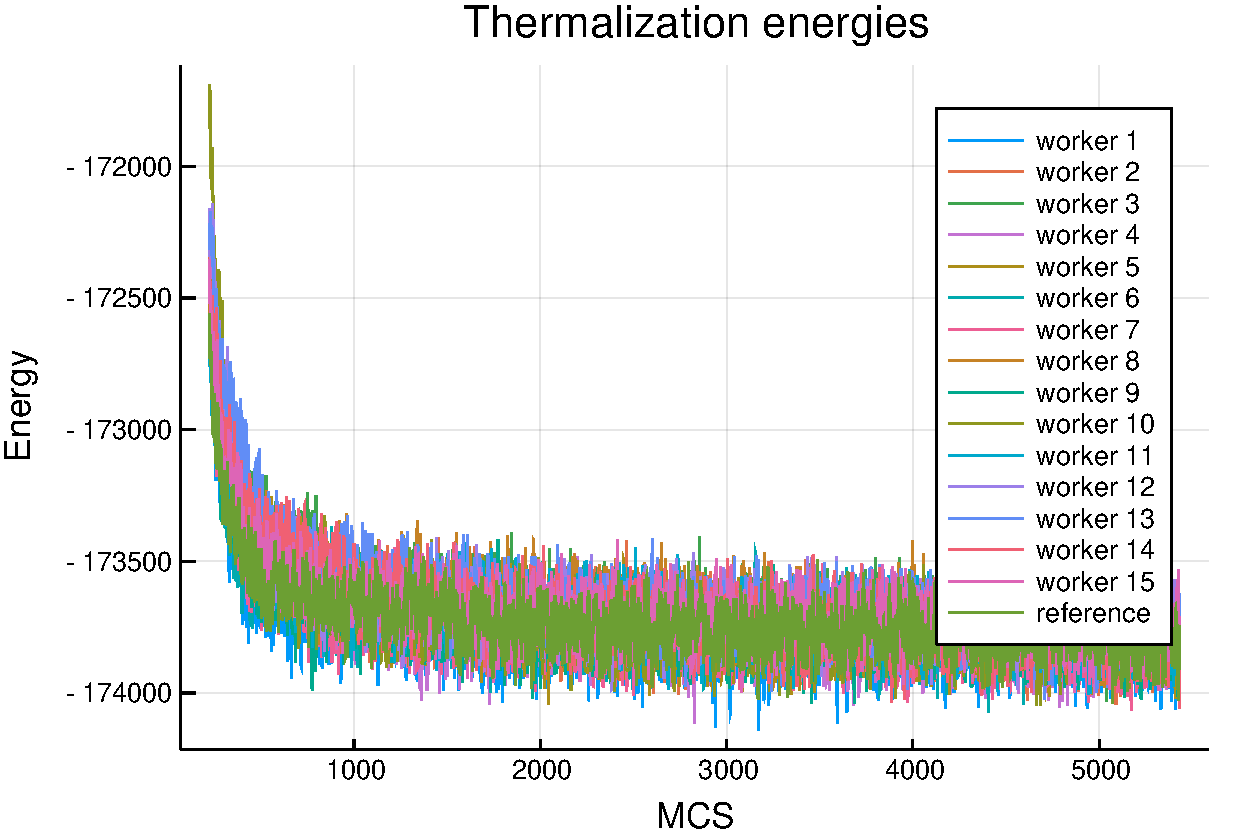
\includegraphics[width=\textwidth]{thermalization_plot_1compXY.pdf}
    \caption{Thermalization of a $64^3$ single-component $XY$-system from random initial states to a numerical temperature $T=0.5$.
    The different curves represent the energy of different realizations of the same
    system initialized at different random states over several \ac{mcs}s. The random initial states have a relatively high energy that stabilizes
    to the same value for all realizations in an exponential fashion.}
    \label{fig:Monte:therm_plot}
\end{figure}

Whether the energy stabilizes from above or below will depend
on what the initial state is and what the temperature of the simulation is set to. For an ab-iniito state, in which the values of the sub-states
are set to uniformly distributed random values in their validity range, this normally corresponds to a very high temperature and
high energy state, hence thermalizing from such a state will have the energy stabilize from above. Another possibility for an ab-inito
state is some kind of mean-field minimal solution of the Hamiltonian where sub-states at different sites are correlated. In this case the
energy will usually be low and the thermalization energy will stabilize from below. This option has the disadvantage that if the mean field
solution lies inside some local energy minimum then simulations based on it might not be able to get out and find the global miniomum,
as opposed to states that are thermalized from high energy where some might find this local minimum while others fall down in the global one.
In general it is best to thermalize several independent systems from different initial conditions that yield quantitatively similar results
to make it less likely that the results come from a local minimum.

A last suggestion for an initial state of the system,
is the last state of a previous simulation. In this case the thermalization will stabilize depending on the relative temperature
of the two simulations. To be sure that the measurements are not correlated with the measurements of the last simulation one should discard
This is a useful practice if gathering results over an extended temperature range where the systems need a large
thermalization time in order to stabilize. One would then typically start measuring at a high temperature and then decrease the temperature
sucessively in steps with a thermalization period and measure period for each step.

For systems prone to fall into local minima it was found that a more careful thermalization period analogous to the measurement procedure 
described above, decreased the probability of freezing into such minima. Instead of thermalizing from a high energy - high temperature state
directly down to the desired temperature, which we call quenching, a cooldown period was added. During the cooldown period, the temperature was
lowered stepwise from a high temperature $T_0$ to a target temperature $T$ with intermediate temperatures
\begin{equation}
    \label{eq:Monte:Therm:geometricTemperatures}
    T_k = \Big(\frac{T}{T_0}\Big)^{\frac{k}{N}}T_0.
\end{equation}
The intermediate temperatures were geometrically distributed to ensure highest density of intermediate steps at lower temperatures. At
each temperature step, a fixed number of \ac{mcs}s were preformed such that more \ac{mcs}s were done towards the lower temperature than
higher. This was done because the simulations in general took longer to thermalize when the temperature decreased. An example of how the
energy changed during such a thermalization period is shown in Figure~\ref{fig:Monte:cooldown_plot}.

\begin{figure}[t]
    \centering
    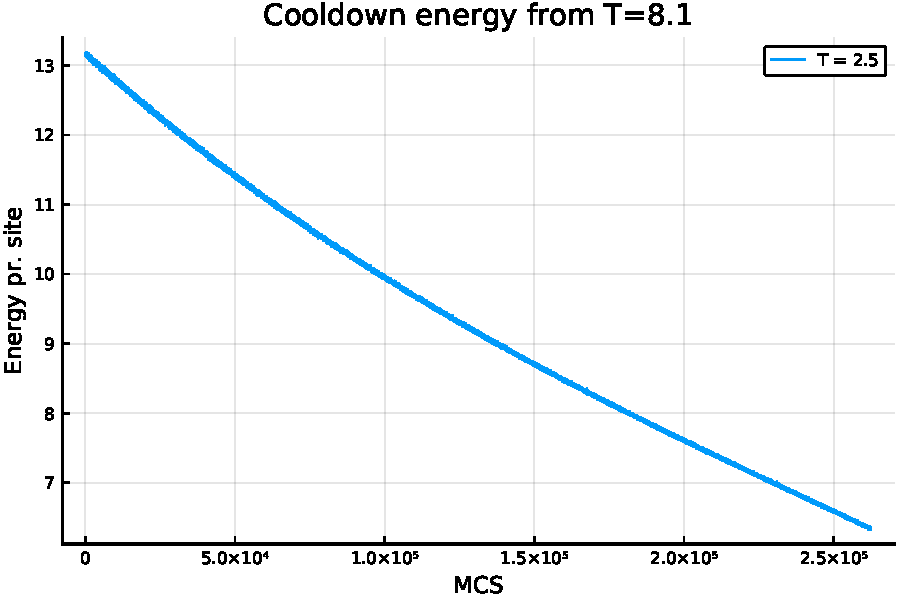
\includegraphics[width=\textwidth]{cooldown_full_model.pdf}
    \caption{Energy pr. site of a $64^3$ site model system of a $p+ip$ chiral superconductor during the cooldown stage. The temperature is
    lowered as a geometric sequence and a fixed number of \ac{mcs}s are done at each temperature step. Comparing with the thermalization
    in Figure~\ref{fig:Monte:therm_plot} we see that the cooldown period gives a significantly more gradual thermalization.}
    \label{fig:Monte:cooldown_plot}
\end{figure}

The cooldown period was then followed by a conventional thermalization stage where the temperature was held constant at $T$. In
most cases the energy had already stabilized at this point such that the energy measurements during this extra thermalization
stage typically only showed fluctuations around the mean.


\section{Parallel tempering}

Parallel tempering is a method of simulating multiple systems over a range of different temperatures where the systems can exchange
positions with their neighbors in this temperature range according to a \ac{mh}-like update step. Since all the different systems all have the same parameters
except for temperature, when viewed from the perspective of a single temperature, this leads to a normal Metropolis-Hastings \ac{mcmc}
simulation with an occational global update of all sites of the system whenever the current system exchanges with the system at a neighboring
temperature. From the dual perspective of a single system, \ac{pt} allows the system to move in temperature space.

This global updating, or movement in temperature space, has the advantage that it can prevent systems from getting stuck in local minima
by allowing them to move to a higher temperature where it is easier to fluctuate to a more favorable configuration. In systems that
has a jagged energy-landscape with lots of local minima this can be of great benefit and can reduce the required time it takes
to measure observables with a certain accuracy by several orders of magnitude \cite{Katzgraber09}.

To implement parallel tempering \ac{mcmc} in a temperature centric perspective,
let $\{T_i\}_{i=1}^M$ be a sorted list of $M$ ascending temperatures, and let $\{\lambda_i\}_{i=1}^M$
be a list of indices $\lambda$, that refer to replica states $\{\psi_\lambda\}_{\lambda=1}^M$ of the system such that the replica with temperature $T_i$
is given by $\psi_{\lambda_i}$ and its energy is given by $E_{\lambda_i}$.
The simulation then proceeds according to the algorithm
\begin{enumerate}
    \item Preform $\Delta t$ normal Monte-Carlo updates on all replica states, \eg using the \ac{mh} method.
    \item For each replica state $\psi_\lambda$ calculate the corresponding energy $E_\lambda$.
    \item For each pair of neighboring temperatures $T_i$ and $T_{i+1}$ where $T_i<T_{i+1}$:
        \begin{enumerate}
            \item calculate the quantity
            \begin{equation}
                \label{eq:Monte:PT:delta}
                \Delta = (E_{\lambda_{i+1}} - E_{\lambda_i})\Big(\frac{1}{T_{i+1}} - \frac{1}{T_i}\Big).
            \end{equation}
            \item Then swap the indices $\lambda_i \leftrightarrow \lambda_{i+1}$ with probability $\min\{1, e^\Delta\}$. This can
                as in the \ac{mh} method be done by generating a random number $r\in[0,1)$ and then swapping indices if
                $\ln r \leq \Delta$.
        \end{enumerate}
    \item If the replicas $\psi_\lambda$ have internal knowledge of their temperatures, then distribute $T_i$ to $\psi_{\lambda_i}$, for all
        temperatures $T_i$.
    \item Sample observables and return to 1.
\end{enumerate}

This algorithm is very efficiently parallelizable since the bulk of computing time will be going to doing the $\Delta t$ \ac{mc} updates which can
be performed in parallel by having each replica state $\psi_\lambda$ be assigned to a separate thread / processor. If each thread in addition
keeps track of the replicas energy at the end of the \ac{mc} updates, the only information that needs to be transferred between worker processes and
the process doing the \ac{pt} update step is the values of the energies to the \ac{pt} process, and afterwards: the set of new temperatures
back to the worker processes. The \ac{pt} process itself only has to 
calculate $M-1$ values and move around the indices in an array.

For the parallel tempering method to generate good statistics efficiently, some care should be taken in the distribution of the temperatures $T_i$.
A rule of thumb is to distribute them geometrically, \ie according to
\begin{equation}
    \label{eq:Monte:PT:geometricTemperatures}
    T_i = \bigg(\frac{T_M}{T_1}\bigg)^{\frac{k-1}{M-1}}T_1,
\end{equation}
with the argument that lower temperatures generally have a lower relaxation rate. With geometric distribution, the temperatures are denser towards
the low end such that the accpetance rate of swaps of replicas at neighboring temperatures would in general become more flat and independent of temperature.
Should the specific heat diverge at some point in the temperature range as in the case of a phase transition, then this distribution would no
longer be optimal since the acceptance probability of temperature swaps is inversely proportional to $C_v$ and thus the accpetance rate would no
longer be flat.

From the perspective of an individual replica, the overall goal with the distribution of temperatures is to maximize the number of the replica moves
from the lowest temperature $T_1$, up to the highest temperature $T_M$ and back to the lowest temperature again. This will then maximize the number
of statistically independent visits of the system at each temperature. The hope then is that a flat accpetance rate with respect to the distributed
temperatures will provide a good number of round-trips. With more advanced methods such as the feedback-optimized parallel-tempering Monte-Carlo
method the number of round-trips can be optimized \cite{Katzgraber06}.

\section{Grid parallelization}

A simple way of utlizing multiple processor cores, or cpus on a multi-cpu system, is to run indipendent monte-carlo simulation on each processor. This
is usually very efficient if a parameter of the system such as temperature is to be varied over some intervall. Then each simulation could have a
different value of this parameter. In this case it is recommended to also implement parallel tempering since the extra overhead is minimal and the
speedup of the simulations can be significant.

Alternatively, all the simulations can run with the same value on different processes and the samples from the individual simulations can then,
be combined to a super-sample. This has the advantage that the individual sampling runs can be shortened and the implementation of the parallelization
is straight-forward. A drawback with this method is however that separate simulations has to be thermalized individually, such that the more the
super-sample is split on different processes, the more processor time is wasted on thermalization. Additionally, if the individual simulation
runs depend on some sort of freezing like how vorticies freeze to the numeric lattice, then individual simulations could freeze at different
angles such that they can not be combined to form good statistics.

\begin{figure}[t]
    \centering
    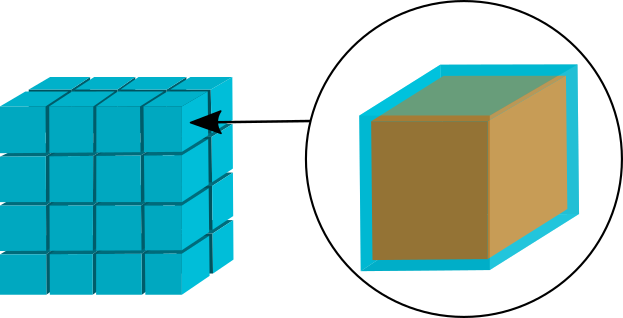
\includegraphics[width=\textwidth]{sub_cuboids.png}
    \caption{Illustration of the sub-division of the numerical grid into sub-cuboids. The right side illustrates that the sites in each sub-cuboid
    can be categorized as either internal sites, which can be updated asynchronuously on different sub-cuboids and is illustrated in the figure
    by the internal orange cube, or sites in a border region.}
    \label{fig:Monte:numerical_grid}
\end{figure}

A solution to the above issues with this simple parallelization is provided by grid-parallelization. This parallelization method is suited for
simulations that consist of interacting sites either in $2$D or $3$D where local Monte-Carlo updates is to be preformed.
We will focus on the case of a $3$D simulation where the sub-sites
are organized in a numerical cubic lattice. The idea is to split the cube into different sub-cuboids as illustrated on the left side of
Figure~\ref{fig:Monte:numerical_grid}. Each sub-cuboids internal sites can then
be updated in the normal Monte-Carlo fashion in parallell with the internal sites of other sub-cuboids. If the individual sites of the original
system interacts with neighboring sites\footnote{In the case of a local \ac{mh} update this can take the form of an energy-difference of
the system at a proposed update-site that depends on the value of fields at neighboring sites.}, then it will be necessary for each sub-cuboid to have
a border whose thickness depends on the range of the interaction. The sites in this border-region will then have an interaction with sites in
the border-region of other sub-cuboids such that care has to be taken not to update a site based on the value of a neighboring site that is no
longer valid. One solution to this is simply updating all the sites in the border-regions serially, \ie update the border sites in a single sub-cuboid,
communicate the updated values to the affected neighboring sub-cuboids, then move to the next sub-cuboid, etc. Or, it could be even more effective
to parallelize the updates of the border sites as well by further sub-dividing the border-sites into different categories. As an example, one could
define internal border-sites on the face of a sub-cuboid to be the border-sites that only depend on sites in the single neighboring sub-cuboid that
is in the direction of the face-plane normal vector. Then all the right-facing internal border-sites can be done in parallel on all sub-cuboids, followed
by all the top-facing internal border-sites, etc.

\section{Reweighting}

Reweigting techniques are methods of finding estimates of parameter-dependent observables at specific parameter values based on previously obtained
samples of these observables from \ac{mc}-simulations that have been done at parameter values independent or the reweighting parameters.
Given a set of samples of some observable $\{o_i\}_{i=1}^M$ from previous \ac{mc} simulation(s), these techniques provide
a set of weights $\{w(\beta')_i\}_{i=1}^M$ that can be used to estimate the observable at a parameter value $\beta'$ by the reweighting
\begin{equation}
    \label{eq:Monte:Reweighting:generalReweighting}
    \hat{o}(\beta') = \sum_iw(\beta')_io_i.
\end{equation}
This is very useful when estimating some observable over a temperature-range since then a single simulation can yield results
not only for a single temperature, but for an extended region. If this region is close to a phase-transition then this can be used as a way of avoiding the
critical slowing down of simulations at phase transitions by instead simulating at temperatures close to the phase-transition and then using reweighting
techniques to estimate results at the phase-transition temperature. All this is possible because a simulation at a given temperature\footnote{It is possible
to use rewighting techniques on other parameters of the simulation as well, as long as they are, like inverse-temperature, linear in the action.}
produces a statistical distribution of energy values for the sampled states. This energy distribution will in general overlap with the energy-distribution
produced when simulating at a temperature that is sufficiently close to the original. Because of this overlap, it is possible to statistically extrapolate
the value of observables at the neighboring temperature.

Reweighting techniques are divided into single-histogram- and multi-histogram reweighting-techniques depending on whether they use statistical information
from a single histogram or can combine histograms generated at multiple parameter values. The single-histogram techniques is used to estimate values of the observables
at neighboring temperature-values and has the virtue of being comparatively simple to implement and understand. The multi-histogram
techniques, on the other hand, has the advantage that the additional statistical information in general gives better estimates and is able to even give better estimates
at the original temperatures the simulations were preformed at, but has a more involved implementation.

In our simulations we used a Julia implementation\footnote{This implementation is available at
\url{https://github.com/Sleort/FerrenbergSwendsenReweighting.jl/tree/1.0.3_update}}
 of the multi-histogram technique originally developed by Bojesen, a technique which they used in \cite{Bojesen13M},
and updated for the current Julia release by us.

\subsection{Ferrenberg-Swendsen single-histogram method}

To derive the Ferrenberg-Swendsen single-histogram reweighting technique, let $o_i$ be samples of an observable $\mathcal{O}$ done at sample states $\psi_i$ of a system
with Hamiltonian $\mathcal{H}$ at parameter value $\beta$, such that $\mathcal{O}(\psi_i) = o_i$.
Then, from out discussion of importance sampling, the estimate of the average of the observable when the states are sampled
according to a probability distribution $\pi(\psi_i)$ is given by
\begin{equation}
    \label{eq:Monte:Reweighting:avgEstimate}
    \langle \hat{\mathcal{O}}\rangle_\beta = \frac{\sum_io_ie^{-\beta\mathcal{H}(\psi_i)}/\pi(\psi_i)}{\sum_ie^{-\beta\mathcal{H}(\psi_i)}/\pi(\psi_i)}.
\end{equation}
Using a simulation with importance sampling at parameter-value $\beta$ to generate the sampled states, the probability distribution was
\begin{equation}
    \label{eq:Monte:Reweighting:probDist}
    \pi(\psi_i) = \frac{e^{-\beta\mathcal{H}(\psi_i)}}{Z_\beta} = \frac{e^{-\beta\mathcal{H}(\psi_i)}}{\sum_\psi e^{-\beta\mathcal{H}(\psi)}},
\end{equation}
where the sum in the denominator is over all possible states $\psi$ and not sampled states. Inserting $\pi(\psi_i)$ into $\langle\mathcal{O}\rangle_\beta$
in Eq.~\eqref{eq:Monte:Reweighting:avgEstimate}, this equation reduces to the arithmetric average, however if we now imagine wanting an estimate of
$\langle\mathcal{O}\rangle_{\beta'}$ at an arbitrary parameter value $\beta'$, then insertion yields
\begin{equation}
    \label{eq:Monte:Reweighting:FS}
    \langle \hat{\mathcal{O}}\rangle_{\beta'} = \frac{\sum_io_ie^{-(\beta'-\beta)\mathcal{H}(\psi_i)}}{\sum_ie^{-(\beta'-\beta)\mathcal{H}(\psi_i)}}.
\end{equation}
This expression then gives an estimate of the average of the observable $\mathcal{O}$ at an arbitrary parameter value $\beta'$ using states $\psi_i$ that
were sampled at a specific parameter value $\beta$. This is called the Ferrenberg-Swendsen single-histogram reweighting technique \cite{FS_1988}, and in terms of the reweighting
expression in Eq.~\eqref{eq:Monte:Reweighting:generalReweighting} we can read off that the weights of this technique are given by
\begin{equation}
    \label{eq:Monte:Reweighting:FS:weights}
    w(\beta')_i = \exp\Big[-\ln\Big(\sum_je^{-(\beta'-\beta)[\mathcal{H}(\psi_j)-\mathcal{H}(\psi_i)]}\Big)\Big].
\end{equation}
Although simple, this techniques ability to extract information about observables around the simulated paramter-value makes it extremely valuable 
in for instance the study of scaling relations or to accurately calculate the peak of thermodynamic variables when the \ac{mc}-simulations themselves take a significant
amount of computing time.

\subsection{Numeric evaluation of exponential sums}
\label{sec:Monte:Reweighting:expSums}

The reason for introducing the extra exponential in the form of $w(\beta')_i$ in Eq.~\eqref{eq:Monte:Reweighting:FS:weights} is because sums of exponential
numbers generally are hard to do numerically using finite-precision
floating point numbers, however the logarithm of such a sum can be found using an iterative scheme. Let $S^{(k)}$ be a sum of $k$
exponential numbers decreasing in magnitude that presumably are too large to be stored individually such that
\begin{equation}
    \label{eq:Monte:Reweighting:FS:expSum}
    S^{(k)} = e^{a_1} + e^{a_2} + \ldots + e^{a_k},
\end{equation}
with $a_{i+1}\leq a_i$, is numerically hard to do. Assuming however that fractions of the numbers can be stored, then we can numerically calculate
\begin{equation}
    \label{eq:Monte:Reweighting:FS:initialLnSum}
    \ln S^{(2)} = a_1 + \ln\Big(1+e^{a_2-a_1}\Big).
\end{equation}
Following the iteration
\begin{equation}
    \label{eq:Monte:Reweighting:FS:iteratedLnSum}
    \ln S^{(k)} = \ln S^{(k-1)} + \ln\Big(1+e^{a_k-\ln S^{(k-1)}}\Big),
\end{equation}
then $\ln S^{(k)}$ can be found for arbitrary $k$ without ever storing a single exponential number, only fractions of such numbers that are close to each other.

\subsection{Multi-histogram Ferrenberg-Swendsen method}

Let $\{\psi_i^k\}_{i=1}^{N_k}$ be sets of states sampled at the $N_0$ inverse temperatures $\beta_k$ of a system with Hamiltonian $\mathcal{H}$.
The energy of these states are then given by $E_i^k$ and samples of an observable $\mathcal{O}$ at these states are given by $\mathcal{O}(\psi_i^k) = o_i^k$.
The energy-samples can then be used to construct $N_0$ histograms
\begin{equation}
    \label{eq:Monte:Reweighting:MFS:interactedLnSum}
    h_k(E) = \sum_{i=1}^{N_k}\delta_{E,E_i^k},
\end{equation}
giving the number of sampled states at a certain energy in the simulation with parameter value $\beta_k$. The goal is to use these histograms to estimate the
density of states of the system which we for the purpose of the derivation of this method will define $n(E) = \sum_\psi\delta_{E,\mathcal{H}(\psi)}$.
The essential steps in this derivation can be found in the original paper in Ref.~\cite{FS_1989}, as well as Ref.~\cite{Newman99} and \cite{rummukainen}.
With these
definitions, the energetic probability distribution of the system at an inverse temperature $\beta$ is given by
\begin{equation}
    \label{eq:Monte:Reweighting:MFS:enProbDist}
    W(\beta,E) = n(E)e^{-\beta E}/Z_\beta,
\end{equation}
where $Z_\beta = \sum_\psi e^{-\beta\mathcal{H}(\psi)}$ is the parition function. Based on the sampled histograms, $W(\beta_k,E)$ at temperature $\beta_k$ can be estimated
by $\hat{p}_k(E) = h_k(E)/N_k$, \ie $\langle\;\hat{p}_k(E)\;\rangle = W(\beta_k,E)$. This implies that $\langle\;h_k(E)\;\rangle = N_kW(\beta_k,E)$ and assuming for now
that the samples of states $\psi_i^k$ and $\psi_j^k$ are statistically independent, it can be shown that 
\begin{equation}
    \label{eq:Monte:Reweighting:MFS:avgHistogramSquared}
    \langle\;h_k(E)^2\;\rangle = N_kW(\beta_k,E)[1 + (N_k-1)W(\beta_k,E)].
\end{equation}
Inserting these cumulants of the histograms into the variance we get
\begin{equation}
    \label{eq:Monte:Reweighting:MFS:histogramVariance}
    \delta^2h_k(E) = \langle\;h_k(E)^2\;\rangle - \langle\;h_k(E)\;\rangle^2 = g_kN_kW(\beta_k,E),
\end{equation}
by assuming $W(\beta_k,E)\ll1$. The factor $g_k = 1+2\tau_k$, where $\tau_k$ is the autocorrelation time of the samples at $\beta_k$, is included to generalize the result
to samples where $\psi_i^k$ and $\psi_j^k$ are not statistically independent.

By solving Eq.~\eqref{eq:Monte:Reweighting:MFS:enProbDist} w.r.t. $n(E)$ and inserting the estimator of $W(\beta_k,E)$, an estimator of the density of states is given by
\begin{equation}
    \label{eq:Monte:Reweighting:MFS:DOSEstimator}
    \hat{n}_k(E) = \hat{p}_k(E)Z_{\beta_k}e^{\beta_kE},
\end{equation}
where $Z_{\beta_k}$ is assumed known, an assumption we have to reconcile later. By the error propagation formula, then the variance of this estimator is given by
\begin{equation}
    \label{eq:Monte:Reweighting:MFS:DOSVariance}
    \delta^2\hat{n}_k(E) = (Z_{\beta_k}e^{\beta_kE}/N_k)^2\delta^2h_k(E).
\end{equation}
The estimator $\hat{n}_k(E)$ is an estimator of $n(E)$ using only a single histogram. We combine the estimators of single histograms using a weighted sum
\begin{equation}
    \label{eq:Monte:Reweighting:MFS:DOSWeightedEstimator}
    \hat{n}(E) = \sum_kr_k\hat{n}_k(E),
\end{equation}
where the coefficients $r_k$ has to satisfy the condition $\sum_kr_k = 1$ for the expectation value of $\hat{n}(E)$ to give the density of states. The coefficients
$r_k$ are determined by minimizing the variance $\delta^2\hat{n}_k(E)$ subject to the constraint $\sum_kr_k=1$ using Lagrange multiplier which yields the estimator
\begin{equation}
    \label{eq:Monte:Reweighting:MFS:minimizedDOSWeightedEstimator}
    \hat{n}(E) = \frac{\sum_{k=1}^{N_0}g_k^{-1}h_k(E)}{\sum_{l=1}^{N_0}N_lg_l^{-1}e^{-\beta_lE}Z_{\beta_l}^{-1}}.
\end{equation}
The assumption that $Z_{\beta_k}$ is known is now reconciled. Since we can write the partition function using the density of states through
\begin{equation}
    \label{eq:Monte:Reweigehting:MFS:partitionFunctionDOS}
    Z_\beta = \sum_\psi e^{-\beta\mathcal{H}(\psi)} = \sum_En(E)e^{-\beta E},
\end{equation}
then we use the density of states estimator to estimate the parition function, and use this estimate of the partition function $\hat{Z}_{\beta_k}$ in the density
of states estimator. This then creates an implicit equation for $\hat{Z}_{\beta_k}$ that has to be solved self-consistently. Inserting the definition of $h_k(E)$
and exchanging sums to remove the histograms, this equation takes the form
\begin{equation}
    \label{eq:Monte:Reweighting:MFS:selfConsistencyEq}
    \hat{Z}_{\beta} = \sum_{k=1}^{N_0}\sum_{i=1}^{N_k}\frac{g_k^{-1}e^{-\beta E_i^k}}{\sum_{l=1}^{N_0}N_lg_l^{-1}e^{-\beta_lE_i^k}\hat{Z}_{\beta_l}^{-1}},
\end{equation}
which gives $N_0$ equations for $N_0$ unknows $\hat{Z}_{\beta_k}$ when evaluated at the different $\beta=\beta_m$.

Solving Eq.~\eqref{eq:Monte:Reweighting:MFS:selfConsistencyEq} is usually done with the help of an iterative solution method for non-linear
equations such as the Newton-Raphson method. To numerically calculate a solution, it is inconventient to work with the full quantities $\hat{Z}_{\beta_m}$
since these are usually extremely large. Instead it is sufficient to calculate the variables
\begin{equation}
    \label{eq:Monte:Reweighting:MFS:logVars}
    L_m \equiv \ln \hat{Z}_{\beta_m} - \ln \hat{Z}_{\beta_1},
\end{equation}
since the weights in the reweighting of observables can be written in terms of them. Dividing Eq.~\eqref{eq:Monte:Reweighting:MFS:selfConsistencyEq} by $Z_{\beta_1}$,
we get that the $N_0-1$ equations we need to solve self consistently for the $N_0-1$ variables $L_m$ are given by
\begin{equation}
    \label{eq:Monte:Reweighting:MFS:modifiedSelfConsistencyEq}
    L_m = \ln\left\{\sum_{k=1}^{N_0}\sum_{i=1}^{N_k}\frac{g_k^{-1}e^{-\beta_mE_i^k}}{\sum_{l=1}^{N_0}g_l^{-1}e^{-\beta_lE_i^k-L_l}}\right\}.
\end{equation}
This form has the big advantage that the overall logarithm allows us to not have to calculate the exponential sums directly, but instead only calculate logarithms
of these sums. For each sum $\sum_ie^{a_i}$ containing exponentials, which are potentially too large to be stored numerically, we simply re-exponentiate the entire
sum to $\exp\ln\sum_ie^{a_i}$ and then use the method outlined in Section~\ref{sec:Monte:Reweighting:expSums} to calculate $\ln\sum_ie^{a_i}$. Because of the
overall logarithm, the exponential drops out in the last re-exponentiation such that we never have to store a single exponential number.

After finding self-consistent values for the $N_0-1$ vairables $L_m$, the weights $w_i^k$ for reweighting the observable $\mathcal{O}$ can be found. In terms of the
density of states $n(E)$, the thermal average of the observable is written
\begin{equation}
    \label{eq:Monte:Reweighting:MFS:obs:thermAvg}
    \langle\mathcal{O}\rangle_\beta = \frac{\sum_E\mathcal{O}(E)n(E)e^{-\beta E}}{\sum_En(E)e^{-\beta E}}.
\end{equation}
Inserting the reweighting estimate of $\hat{n}(E)$ in Eq.~\eqref{eq:Monte:Reweighting:MFS:minimizedDOSWeightedEstimator} for $n(E)$ we get the reweighting estimate
\begin{equation}
    \label{eq:Monte:Reweighting:MFS:obs:reweightedThermAvg}
    \langle\hat{\mathcal{O}}\rangle_\beta = \frac{\hat{Z}_{\beta_1}}{\hat{Z}_\beta}\sum_{k=1}^{N_0}\sum_{i=1}^{N_k}\frac{o_i^kg_k^{-1}e^{-\beta E_i^k}}{\sum_{l=1}^{N_0}N_lg_l^{-1}e^{-\beta_lE_i^k-L_l}},
\end{equation}
where $\hat{Z}_{\beta_1}/\hat{Z}_\beta$ is given by
\begin{equation}
    \label{eq:Monte:Reweighting:MFS:obs:ZFraction}
    \frac{\hat{Z}_\beta}{\hat{Z}_{\beta_1}} = \sum_{k=1}^{N_0}\sum_{i=1}^{N_k}\frac{g_k^{-1}e^{-\beta E_i^k}}{\sum_{l=1}^{N_0}N_lg_l^{-1}e^{-\beta_lE_i^k - L_l}},
\end{equation}
through Eq.~\eqref{eq:Monte:Reweighting:MFS:selfConsistencyEq}. The two equations for $\langle\hat{\mathcal{O}}\rangle_\beta$ in
Eqs.~\eqref{eq:Monte:Reweighting:MFS:obs:reweightedThermAvg} and \eqref{eq:Monte:Reweighting:MFS:obs:ZFraction} together with the self-consistency equation in
Eq.~\eqref{eq:Monte:Reweighting:MFS:modifiedSelfConsistencyEq}, is sufficient to describe the multi-histogram method. Notice that in these equations the
histograms on which the method was derived do not figure but have been replaced by the more fundamental energy samples. This form makes the method more convenient
to implement for systems with continuous energy distributions since it removes the need for a sum over all possible energies.

When calculating the exponential sums in the weights implied by
Eqs.~\eqref{eq:Monte:Reweighting:MFS:obs:reweightedThermAvg} and \eqref{eq:Monte:Reweighting:MFS:obs:ZFraction}, numerical overflow can be avoided by first using
logarithms to calculate the logarithm of a set of related un-normalized weights as before, then subtracting the maximum logarithmic value for each weight such that
each weight is $\lesssim1$ and then using the sum of these weights to properly normalize in the end.

\subsection{Initial guess}

An iterative non-linear solver usually needs an initial guess at the solution. In the case of the multi-histogram method equations,
a good initial guess can be provided by the single-histogram Ferrenberg-Swendsen
method. Since only fractions of partition function values are needed we may set that $\hat{Z}_{\beta_1}=1$ and use the Ferrenberg-Swendsen method based on
the $\beta_1$ energies to estimate the value $\hat{Z}_{\beta_2}^0$ of $\hat{Z}_{\beta_2}$ at neighboring inverse-temperature $\beta_2$ by the formula
\begin{equation}
    \label{eq:Monte:Reweighting:MFS:guess:Zb2}
    \hat{Z}_{\beta_2}^0 = \sum_{i=1}^{N_1}e^{-(\beta_2-\beta_1)E^1_i}.
\end{equation}
In terms of the numerically convenient variables $L_m$ then this first guess $L_{2}^0$ takes the form
\begin{equation}
    \label{eq:Monte:Reweighting:MFS:guess:L2}
    L_{2}^0 = \ln\Big[\frac{1}{N_1}\sum_{i=1}^{N_1}e^{-(\beta_2-\beta_1)E_i^1}\Big].
\end{equation}
Continuing to estimate the partition function $\hat{Z}_{\beta_m}$ through the single-histogram Ferrenberg-Swendsen method based on the data at $\beta_{m-1}$,
then we may find all subsequent $L_{m}^0$ by applying the iteration scheme
\begin{equation}
    \label{eq:Monte:Reweighting:MFS:guess:LIteration}
    L_{m}^0 = L_{m-1}^0 + \ln\Big[\frac{1}{N_{m-1}}\sum_{i=1}^{N_{m-1}}e^{-(\beta_m-\beta_{m-1})E_i^{m-1}}\Big].
\end{equation}

